\section{Experiments}

\subsection{Dataset}
Dataset and experiment desig.

\subsection{Experiment Setup}

\subsubsection{Algorithms}
We compared the results of our framework (\textbf{APART}) with two other approaches; \textbf{SP} (i.e., Shortest Path) and \textbf{NN} (i.e., Nearest Neighbor).

Our implementation of SP is based on the algorithms in \cite{Huang14}. The only advantage of \cite{Huang14} over \cite{Ma13} is the the former considers reordering of the schedule while the latter does not. Although it is shown the performance increase of reordering requests is minimal, since we consider request reordering in APART, we decided to base the SP implementation on algorithms in \cite{Huang14} to make the comparison as fair as possible.

Also, the NN algorithm is implemented based on the current approach adopted by major ridesharing platforms such as Uber. The NN approach, finds the first nearest driver to the pick-up location of a new request. If the driver is able to fit the new request in its schedule without violating any constraints, he accepts the request. Otherwise the request is rejected and the algorithm tries to assign the request to the next nearest driver. This continues until a driver accepts the request of every driver rejects it in which case the request is dropped.

As a result, we are comparing the performance of APART with state-of-the-art approaches from both academia (SP) and industry (NN).

In the first set of experiments, we use the pricing model explained in \cref{subsec:pricing} and compare the three approaches. In ...... we utilize the pricing model introduced in \cite{Ma15} for both APART and SP. In the pricing model of \cite{Ma15}, there is no concept of \textit{revenue} similar to what we introduces in \cref{subsec:pricing}. Therefore, in order to compare the generated revenue, we assume each driver has to pay 20\% of what they make as the server's share.

\subsubsection{Configurations and Measures}
In our experiments we measure three different metrics by varying different parameters of the system. We measure (1) service rate as the percentage of requests that were completed, (2) the revenue of the system and (3) the response time for matching a request with a driver. Also, \cref{tab:params} shows the different values we used for various parameters to evaluate our framework (default values are shown in \textbf{bold}).

\TODO{mohammad}{Write default values for rider and driver profiles}

\begin{table}
\begin{center}
\begin{tabular}{|c|c|}
	\hline
	Parameter & Values \\
	\hline \hline
	Max Wait Time & 3min, \textbf{6min}, 9min, 12min, 15min, 20min \\ 
	\hline
	\# of Drivers & 1000, 2000, \textbf{5000},  10000, 20000\\ 
	\hline
	Max Passengers & 2, 3, \textbf{4}, 5, 6 \\
	\hline
	Max Allowed Detour & 25\%, \textbf{50\%}, 75\%, 100\%\\
	\hline
\end{tabular}
\caption{Parameters for Algorithm Comparison}
\label{tab:params}
\end{center}
\end{table}

\subsection{Algorithm Comparison}
In this section, we evaluate the performance of the three approaches by varying one of the parameters based on \cref{tab:params} while other parameters have their default values. We show how the algorithms compare to each other with regard to service rate, generated revenue and response time.

\subsubsection{Service Rate}
In the first set of experiments we compare the service rate of the three approaches. As shown in \cref{fig:sr}, all algorithms generate high service rates when the constraints are loosened or there is high resource availability. However, under tight constraints or limited resources, APART outperform the other two approaches by up to 20\%. To better explain the reason why APART has a higher service rate, we use the notion of \textit{eligible drivers} defined in \cref{subsec:dispatch}. \TODO{mohammad}{add a chart that shows the percentage of requests where in APART there are more eligible drivers}.

\begin{figure}[h]
    \centering
    \subfigure[\small{Maximum Wait Time}]{
        \label{fig:mwt_sr}
        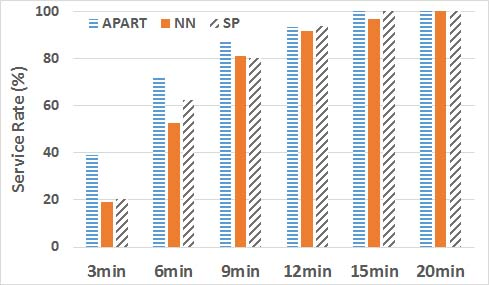
\includegraphics[width = 0.45\columnwidth]{fig/mwt_sr.jpg}
    }
    \subfigure[\small{Number of Drivers}]{
        \label{fig:nd_sr}
        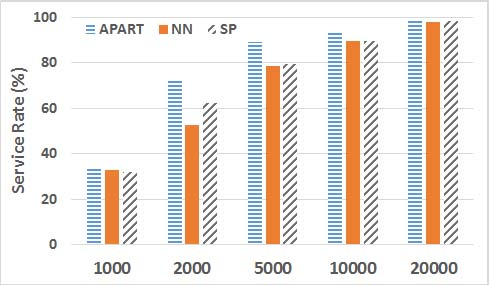
\includegraphics[width = 0.45\columnwidth]{fig/nd_sr.jpg}
    }
    \subfigure[\small{Maximum Passengers}]{
        \label{fig:mp_sr}
        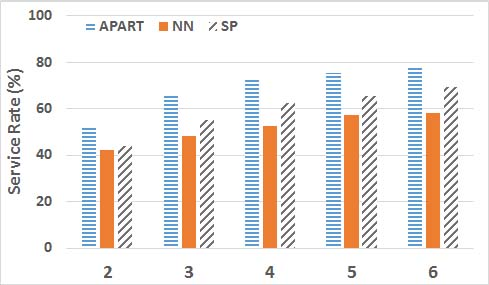
\includegraphics[width = 0.45\columnwidth]{fig/mp_sr.jpg}
    }
    \subfigure[\small{Maximum Allowed Detour}]{
        \label{fig:mad_sr}
        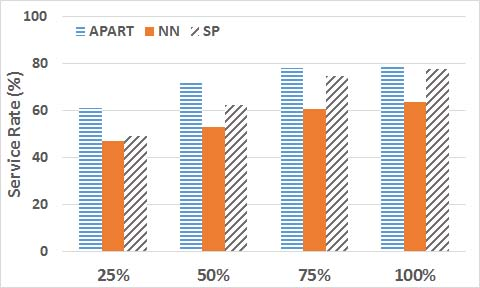
\includegraphics[width = 0.45\columnwidth]{fig/mad_sr.jpg}
    }
    \vspace{-0.15in}
    \caption{Comparing Service Rate of the Algorithms}
    \label{fig:sr}
\end{figure}

\subsubsection{Revenue}
As mentioned, the main objective of APART is to maximize the ridesharing platform's revenue. In these set of experiments, we compare the generated revenue of each algorithm. In these experiments we applied the pricing model explained in \TODO{mohammad}{ref to correct section} and used for the riders and drivers, used profiles similar to the ones in \TODO{mohammad}{ref to sample rider profiles} and \TODO{mohammad}{ref to sample driver profile} respectively. Here, we want to evaluate the effect of varying the parameters in \cref{tab:params} on the overall revenue and compare different algorithms. Later in \cref{subsec:pricingexp} we will apply different pricing models to the algorithms and compare revenue under different pricing models as well.

\begin{figure}[h]
    \centering
    \subfigure[\small{Maximum Wait Time}]{
        \label{fig:mwt_rev}
        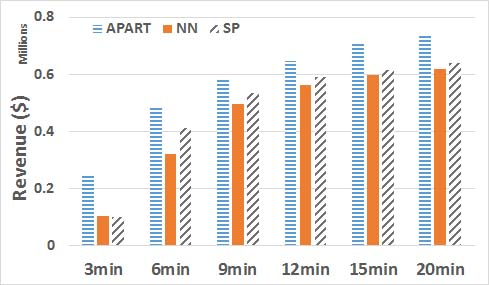
\includegraphics[width = 0.45\columnwidth]{fig/mwt_rev.jpg}
    }
    \subfigure[\small{Number of Drivers}]{
        \label{fig:nd_rev}
        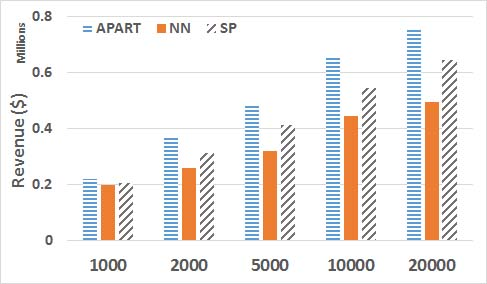
\includegraphics[width = 0.45\columnwidth]{fig/nd_rev.jpg}
    }
    \subfigure[\small{Maximum Passengers}]{
        \label{fig:mp_rev}
        \includegraphics[width = 0.45\columnwidth]{fig/mp_rev.jpg}
    }
    \subfigure[\small{Maximum Allowed Detour}]{
        \label{fig:mad_rev}
        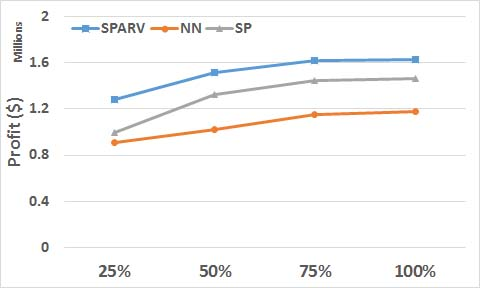
\includegraphics[width = 0.45\columnwidth]{fig/mad_rev.jpg}
    }
    \vspace{-0.15in}
    \caption{Comparing Revenue of the Algorithms}
    \label{fig:rev}
\end{figure}

As it can be seen in \cref{fig:rev} regardless of the values of different parameters, APART generates more revenue than any other approach. When we compare the results in \cref{fig:rev} with the ones in \cref{fig:sr}, even under configurations where all algorithms have the same service rate, APART manages to generate at least 10\% more revenue. The main reason for higher revenue is that APART is designed to make a \textit{Price-aware} assignment, i.e., assign the request to a driver that generates the most profit. Of course, as explained in \TODO{mohammad}{ref to pricing model section}, the pricing models that are used in APART are designed such that the higher profits are not gained by scamming the riders. On the other hand, as it was explained earlier, the SP and NN algorithm were not designed to maximize revenue. An interesting observation in \cref{fig:nd_ref} is that as more drivers are added, the profit decreases even though the service rate increases (\cref{fig:nd_sr}). The NN algorithm gives priority to drivers that are closer to the pick-up location of a request. As long as the driver is able to fit the request in its current schedule without violating the wait time and maximum detour constraints of any request, the request will be assigned to him. This means under certain conditions the sum of discounts other riders will receive can potentially be higher than the final fare of the new request and hence, the system will end up loosing money.

\subsubsection{Response Time}

Similar to \cite{Ma13,Huang14}, APART processes the requests, one request at a time once a request is submitted. In order to evaluate the scalability of our framework, our next set of experiments evaluate the response time of processing a single request. To count for the communication cost of these algorithms, for every message transfer, we add the communication cost as the \textit{message size} divided by a transmission rate of 1Mbit/sec (this is even less than the average speed of a 3G cellular network). \cref{fig:rp} compares the response time of the algorithms under different configurations.

\begin{figure}[h]
    \centering
    \subfigure[\small{Maximum Wait Time}]{
        \label{fig:mwt_rp}
        \includegraphics[width = 0.45\columnwidth]{fig/mwt_rp.jpg}
    }
    \subfigure[\small{Number of Drivers}]{
        \label{fig:nd_rp}
        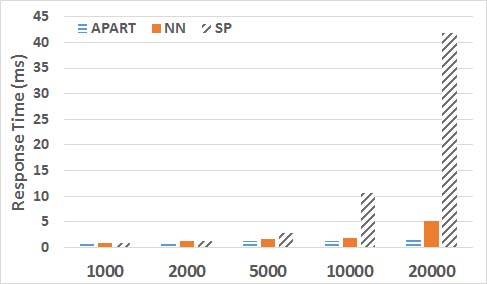
\includegraphics[width = 0.45\columnwidth]{fig/nd_rp.jpg}
    }
    \subfigure[\small{Maximum Passengers}]{
        \label{fig:mp_rp}
        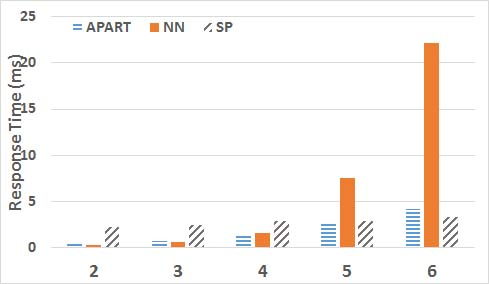
\includegraphics[width = 0.45\columnwidth]{fig/mp_rp.jpg}
    }
    \subfigure[\small{Maximum Allowed Detour}]{
        \label{fig:mad_rp}
        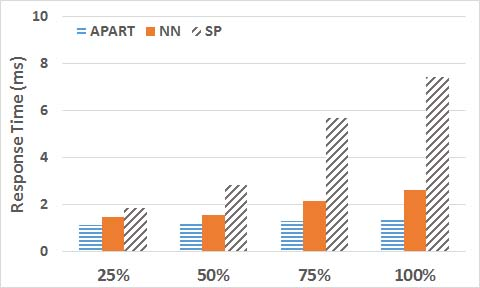
\includegraphics[width = 0.45\columnwidth]{fig/mad_rp.jpg}
    }
    \vspace{-0.15in}
    \caption{Comparing Revenue of the Algorithms}
    \label{fig:rp}
\end{figure}

In \cref{fig:mwt_rp}, the response time increases as more wait time is allowed. This is expected as more wait time, allows drivers to schedule more requests simultaneously which makes the scheduling more time consuming. However, all approaches manage to keep the response time less than 3ms which is acceptable for a real-time framework. However, in \cref{fig:nd_rp}, when more drivers are added, the scalability of SP suffers as it has to perform scheduling for a larger number of vehicles. On the other hand, due to the distributed nature of APART's auction-based approach, each driver does scheduling for itself and adding drivers does not affect the overall response time of APART as much. In \cref{fig:mp_rd} we notice that although APART's response time does not go beyond 2ms, SP handles the increase in maximum passengers better due to the Kinetic Tree structure implementation \cite{Huang14}. The reason for NN's poor performance in \cref{fig:mp_rp} is that it has to \textit{sequentially} perform a computation heavy scheduling, for possibly multiple drivers.

\subsection{Comparing Pricing Models}
\label{subsec:pricingexp}
